\documentclass[a4paper]{article}

\usepackage[english,czech]{babel} %https://github.com/michal-h21/biblatex-iso690
\usepackage[
   backend=biber      % if we want unicode 
  ,style=iso-numeric % or iso-numeric for numeric citation method          
  ,babel=other        % to support multiple languages in bibliography
  ,sortlocale=cs_CZ   % locale of main language, it is for sorting
  ,bibencoding=UTF8   % this is necessary only if bibliography file is in different encoding than main document
]{biblatex}
\usepackage[utf8]{inputenc}
\usepackage{fancyhdr}
\usepackage{amsmath}
\usepackage{amssymb}
\usepackage[left=2cm,right=2cm,top=2.5cm,bottom=2.5cm]{geometry}
\usepackage{graphicx}
\usepackage{pdfpages}
\usepackage{url}
\usepackage{float}

\graphicspath{graficos}

\newfloat{customgraph}{Hn}{grp}
\floatname{customgraph}{Graf}

\floatstyle{plaintop}
\newfloat{customtables}{Hn}{tbl}
\floatname{customtables}{Tabulka}

\pagestyle{fancy}
\lhead{Praktikum I - (VII) Studium kmitů vázaných oscilátorů}
\rhead{Vladislav Wohlrath}
\author{Vladislav Wohlrath}

\bibliography{source}

\begin{document}

\begin{titlepage}
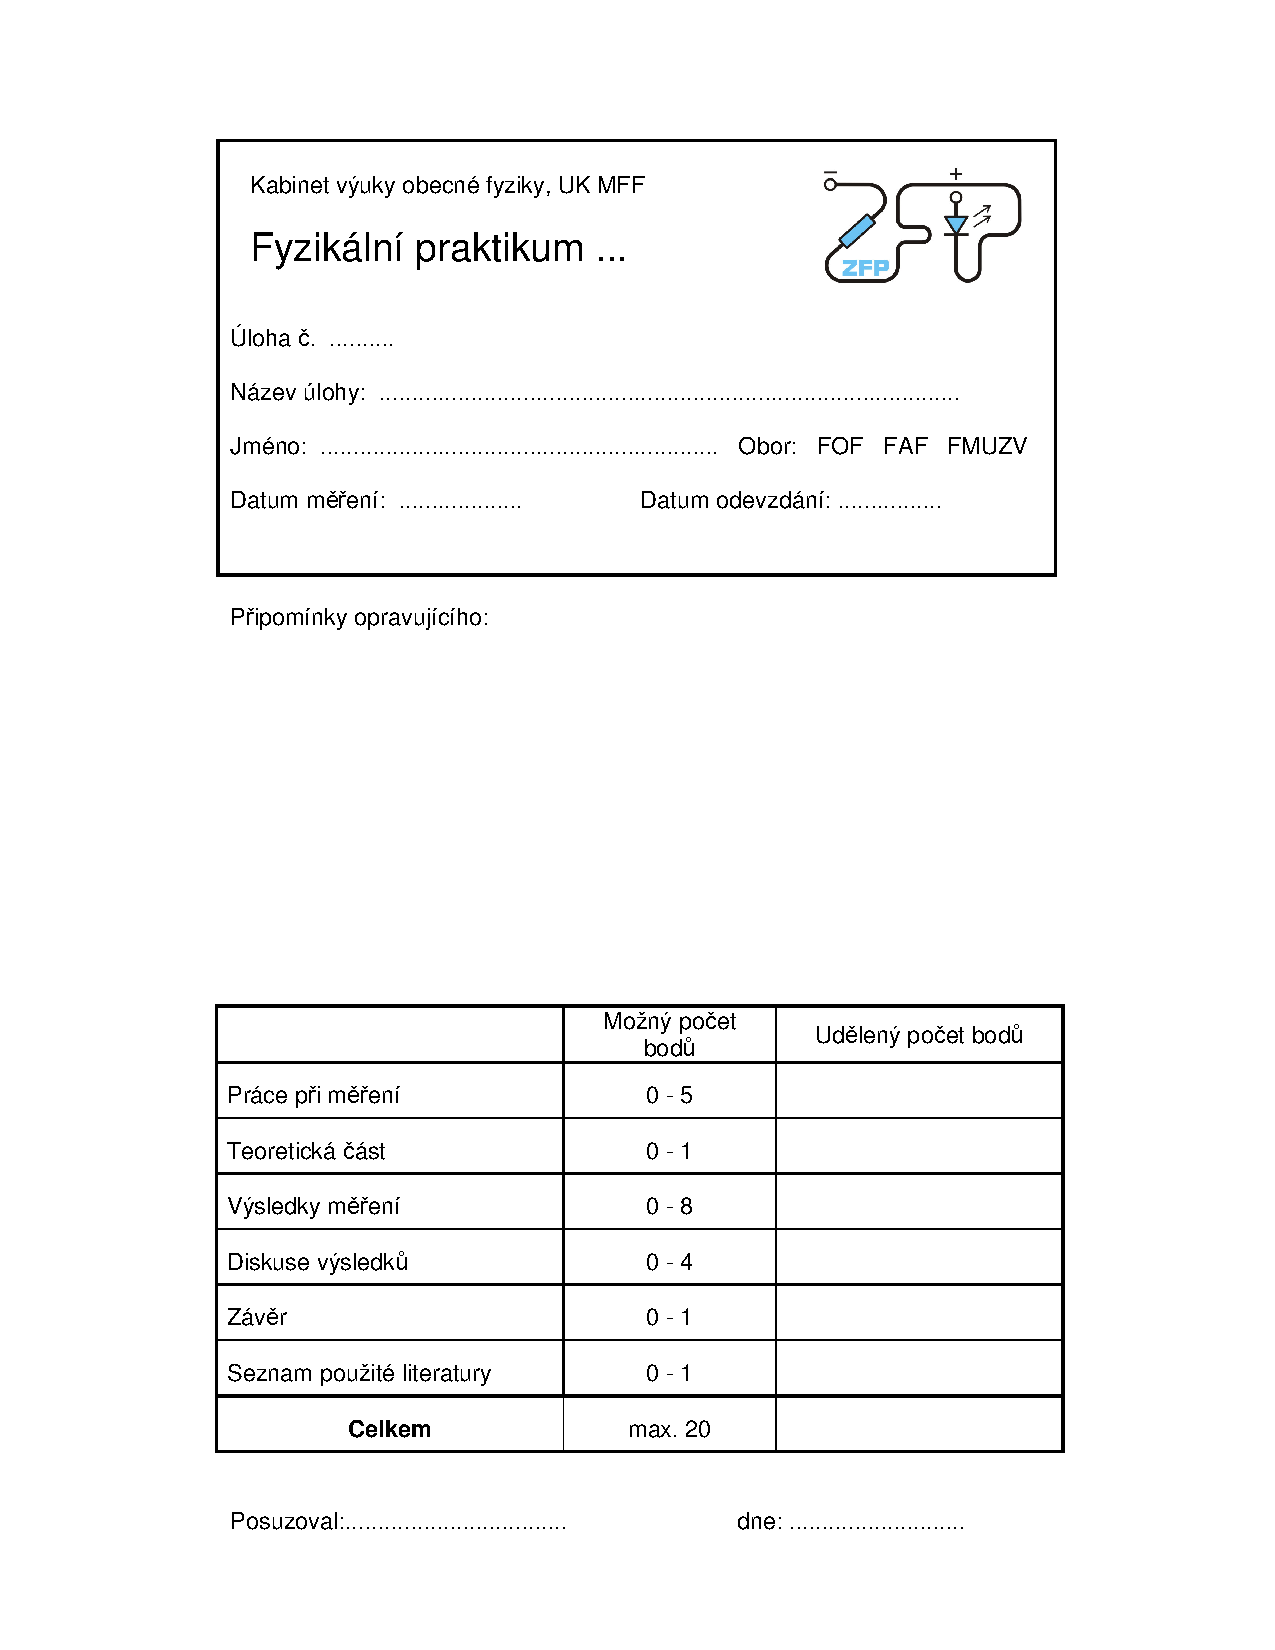
\includepdf[pages={1}]{./graficos/titlelist.pdf}
\end{titlepage}

\section*{Pracovní úkoly}
\begin{enumerate}
\item Změřte dobu kmitu $T_0$ dvou stejných nevázaných fyzických kyvadel.
\item Změřte doby kmitů $T_i$ dvou stejných fyzických kyvadel vázaných slabou pružnou vazbou vypouštěných z klidu při počátečních podmínkách
\begin{enumerate}
\item $y_1=y_2=B$ \ldots doba kmitu $T_1$
\item $y_1=-y_2=B$ \ldots doba kmitu $T_2$
\item $y_1=0, y_2=B$
	\begin{enumerate}
	\item doba kmitu $T3$
	\item doba $T_S/2$, za kterou dojde k maximální výměně energie mezi kyvadly
	\end{enumerate}
\end{enumerate}
\item Vypočtěte kruhové frekvene $\omega _0$, $\omega _1$, $\omega _2$, $\omega _3$ a $\omega _4$ odpovídající dobám $T_0$, $T_1$, $T_2$, $T_3$ a $T_S$, ověřte měřením platnost vztahů odvozených pro $\omega _3$ a $\omega _4$.
\item Vypočtěte stupeň vazby $\kappa$.
\item Pro jednu pružinu změřte závislost stupně vazby na vzdálenosti zavěšení pružiny od uložení závěsu kyvadla a graficky znázorněte.
\end{enumerate}

%Teoretická část
\section*{Teoretická část}
Budeme studovat kmity dvou fyzických kyvadel vázaných slabou pružinou upevněnou ve vzdálenosti $l$ od uložení závěsů kyvadel (viz obrázek \ref{obr::aparatura}).
Po upevnění pružiny se rovnovážná poloha obou kyvadel vychýlí ze svislého směru o úhel $\alpha$ směrem k sobě.
Okamžitou výchylku $\varphi _1(t)$ resp. $\varphi _2 (t)$ uvažujeme od této nové rovnovážné polohy.

\begin{figure}[htbp]
\centering
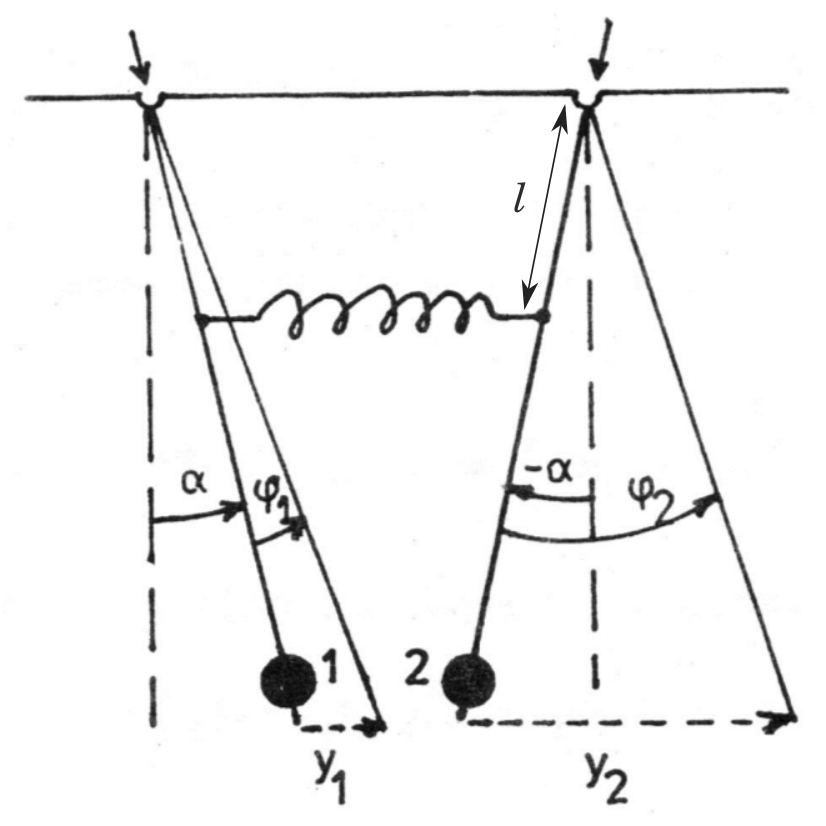
\includegraphics[width=\textwidth-9cm]{graficos/aparatura}
\caption{Nákres experimentu (přezato z \cite{ZFP})}
\label{obr::aparatura}
\end{figure}

Po vyřešení pohybových rovnic dostáváme pro malé výchylky \cite{ZFP}
\begin{align}
\label{eq::phiobecne}
\begin{split}
 \varphi _1(t) &= a_1 \cos (\omega _1 t) + b_1 \sin (\omega _1 t) + a_2 \cos (\omega_2 t) + b_2 \sin(\omega_2 t)
\\
 \varphi _2(t) &= a_1 \cos (\omega _1 t) + b_1 \sin (\omega _1 t) - a_2 \cos (\omega_2 t) - b_2 \sin(\omega_2 t) \,,
\end{split}
\end{align}
kde $a_1$, $b_1$, $a_2$ a $b_2$ jsou integrační konstanty, které určíme z~počátečních podmínek.
Úhlové frekvence $\omega _1$ a $\omega _2$ můžeme vypočítat podle vzorce \cite{ZFP}
\begin{align}
\label{eq::omegadirekcni}
\begin{split}
 \omega_1 &= \sqrt{\frac{D}{I}}
\\
 \omega_2 &= \sqrt{\frac{D+2D^{\ast}}{I}} \,,
\end{split}
\end{align}
kde $I$ je moment setrvačnosti kyvadla, $D$ je direkční moment kyvadla a $D^{\ast}$ je direkční moment pružiny. Žádnou z~těchto veličin však nebudeme měřit a úhlové rychlosti $\omega _1$ a $\omega _2$ změříme přímo při vhodně zvolených počátečních podmínkách.

Pro různé počáteční podmínky vychází:
\begin{enumerate}
\item Pro $\varphi _1 (0) = \varphi _2 (0) = A$, $\dot{\varphi_1}(0)=\dot{\varphi_2}(0)=0$ dostáváme
\begin{equation} \label{eq::philist1}
\varphi _1 = \varphi _2 = A \cos(\omega _1 t)\,.
\end{equation}
\item Pro $\varphi _1 (0) = - \varphi _2 (0) = A$, $\dot{\varphi_1}(0)=\dot{\varphi_2}(0)=0$ dostáváme
\begin{equation} \label{eq::philist2}
\varphi _1 = - \varphi _2 = A \cos(\omega _2 t) \,.
\end{equation}
\item Pro $\varphi _1 (0) = 0$, $\varphi _2 (0) = A$, $\dot{\varphi_1}(0)=\dot{\varphi_2}(0)=0$ dostáváme
\begin{align}
\label{eq::philist3}
\begin{split}
 \varphi_1 &= A \sin(\omega_4 t) \cdot \sin(\omega_3 t)
\\
 \varphi_2 &= A \cos(\omega_4 t) \cdot \cos(\omega_3 t) \,,
\end{split}
\end{align}
kde
\begin{align}
\label{eq::omega34}
\begin{split}
 \omega_3 &= \frac{1}{2}(\omega_2 + \omega_1)
\\
 \omega_4 &= \frac{1}{2}(\omega_2 - \omega_1) \,.
\end{split}
\end{align}

Pokud je vazba slabá, je $\omega _2$ jen o málo větší než $\omega_1$ a pohyb kyvadel můžeme považovat za harmonický s~úhlovou frekvencí $\omega_3$ a v čase proměnnou amplitudou $A \sin(\omega_4 t)$ ($A \cos(\omega_4 t)$ pro druhé kyvadlo). 

\end{enumerate}

Pro úhlové rychlosti $\omega_1$, $\omega_2$ a $\omega_3$ označíme odpovídající periody $T_1$, $T_2$ a $T_3$ resp.
Dále zavedeme dobu $T_S$ jako polovinu periody odpovídající $\omega_4$. Platí tedy vztahy
\begin{align}
\label{eq::periodyvztahy}
 T_1 \omega_1 &= 2\pi & T_2 \omega_2 &=2\pi \nonumber \\
 T_3 \omega_3 &= 2\pi & T_S \omega_4 &=\pi
\end{align}

Standardní odchylku úhlové rychlosti počítáme vždy jako $\sigma_\omega=\omega \cdot \sigma_T / T$.

S nahlédnutím do \eqref{eq::philist3} je $T_S$ zřejmě doba mezi dvěma časy, kdy je amplituda kyvadla nulová (viz~obrázek~\ref{obr::tretipripad}).

\begin{figure}[htbp]
\centering
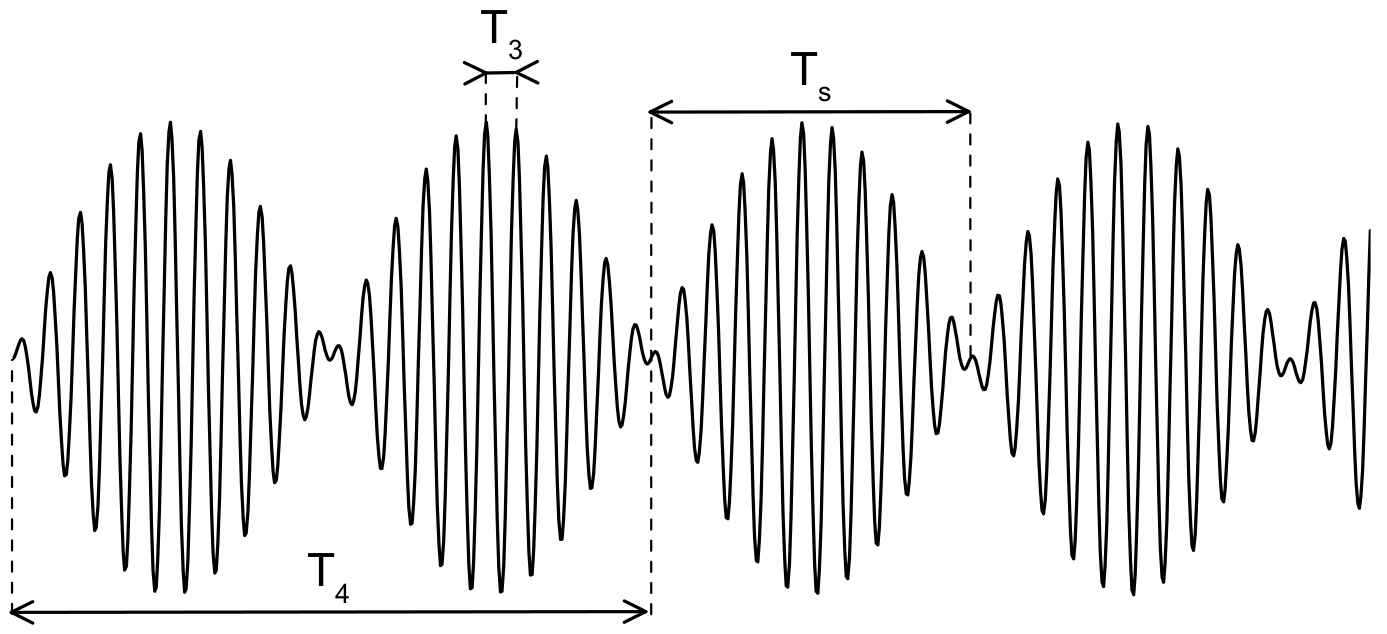
\includegraphics[width=\textwidth-2cm]{graficos/ts}
\caption{Časová závislost výchylky prvního kyvadla $\varphi_1$ při počátečních podmínkách $\varphi_1(0)=0$, $\varphi_2(0)=A$ a $\dot{\varphi_1}(0)=\dot{\varphi_2}(0)=0$, pokud zanedbáme tlumení. Závislost $\varphi_2$ je oproti $\varphi_1$ posunutá o čas $T_S/2$. Doba $T_4$ je perioda odpovídající úhlové rychlosti $\omega_4$ a platí $T_4=2T_S$. (převzato z \cite{ZFP})}
\label{obr::tretipripad}
\end{figure}

Stupeň vazby $\kappa$ je definován jako \cite{ZFP}
\begin{equation} \label{eq::kappadirekcni}
\kappa = \frac{D^{\ast}}{D+D^{\ast}} \,.
\end{equation} 

S využitím \eqref{eq::omegadirekcni} můžeme \eqref{eq::kappadirekcni} upravit na
\begin{equation}
\kappa = \frac{\omega_2^2-\omega_1^2}{\omega_2^2+\omega_1^2} \,.
\end{equation}

Standardní odchylku stupně vazby $\sigma_\kappa$ v závislosti na odchylkách $\sigma _{\omega_1}$ a $\sigma _{\omega_2}$ určíme jako
\begin{equation} \label{eq::odchylkakappa}
\sigma _\kappa = \sqrt{ \left( \frac{\partial \kappa}{\partial \omega_1} \right) ^2 \cdot \sigma_{\omega_1}^2    +   \left(  \frac{\partial \kappa}{\partial \omega_2}     \right)^2 \cdot \sigma_{\omega_2}^2    } = \frac{4 \omega_1^2 \omega_2^2}{ \left( \omega_1^2+\omega_2^2 \right) ^2} \sqrt{ \left( \frac{\sigma _{\omega_1}}{\omega_1}      \right)^2    +      \left( \frac{\sigma _{\omega_2}}{\omega_2}      \right)^2                   }
\end{equation}



%Podmínky a měřící přístroje
\subsection*{Měřící přístroje}
Vzdálenost upevnění pružiny od uložení závěsů kyvadla $l$ jsme měřili svinovacím metrem s nejmenším dílkem \SI{1}{\mm}. Standardní odchylku $\sigma_l$ odhadujeme také na \SI{1}{\mm}.
Dobu kyvu jsme měřili sonarem, který snímal polohu kyvadla v čase se vzorkovací frekvencí \SI{25}{\Hz}. Výstup jsme zobrazili v programu Logger Lite a odečetli dobu většího počtu kyvů (většinou 9 nebo 10). Standardní odchylku určení času odhadujeme na \SI{0,1}{\s}. Protože jsme odečítali dvě hodnoty od sebe, považujeme standardní odchylku změřeného času za $\sqrt{2}\cdot$ \SI{0,1}{\s}. Pokud jsme měřili dobu $n$ kyvů, považujeme za standardní odchylku $\frac{1}{n} \sqrt{2} \cdot$\SI{0,1}{\s}. Uvádíme pouze výsledné časy a jejich odchylky.
Co se týče doby $T_S$, měřili jsme vždy pouze polovinu periody (tedy přímo dobu $T_S$), protože energické ztráty byly příliš vysoké a po dvou periodách byl již celý systém téměř v klidu. Navíc přesný čas, kdy byla amplituda nulová bylo obtížné přesně určit (viz obrázek \ref{obr::tretipripad}). Vzhledem k těmto skutečnostem odhadujeme standardní odchylku $\sigma_{T_S}$ vždy na \SI{0,3}{s}.

%Výsledky měření
\section*{Výsledky měření}
Nejdříve jsme změřili periodu obou kyvadel, když nebyly vázány, abychom se ujistili, že skutečně kmitají stejně.
Naměřené $T_0$ a odpovídající $\omega_0 = 2\pi / T_0$ jsou uvedeny v tabulce \ref{tab::nevazany}.

\begin{tabulka}[htbp]
\centering
\begin{tabular}{ccc}

kyvadlo & $T_0$ (\si{\s}) & $\omega_0$ (\si{\per\second})  \\ \hline
levé & 0 & 0 \\
pravé & 0 & 0 \\
\end{tabular}
\caption{Kmity nevázáných kyvadel}
\label{tab::nevazany}
\end{tabulka}

Časy $T_1$, $T_2$, $T_3$ a $T_S$ jsme změřili s dvěma pružinami A ($k=$~\SI{7}{\newton\per\metre}) a B ($k=$~\SI{4}{\newton\per\metre}) při $l=$~\SI{27,8(1)}{\cm}.
Spolu s odpovídajícími $\omega_1$, $\omega_2$, $\omega_3$ a $\omega_4$ a vypočtenými $\kappa$ jsou uvedeny v tabulce \ref{tab::vsechnyomegy}.

\begin{tabulka}[htbp]
\centering
\begin{tabular}{cccccccccc}

pružina & $T_1$ (\si{\s}) & $\omega_1$ (\si{\per\second})  & $T_2$ (\si{\s}) & $\omega_2$ (\si{\per\second}) & $T_3$ (\si{\s}) & $\omega_3$ (\si{\per\second}) & $T_S$ (\si{\s}) & $\omega_4$ (\si{\per\second}) & $\kappa$ \\ \hline
A & 0 & 0 & 0 & 0 & 0 & 0 & 0 & 0 & 0 \\
B & 0 & 0 & 0 & 0 & 0 & 0 & 0 & 0 & 0 \\
\end{tabular}
\caption{Kmity vázaných kyvadel při různých počátečních podmínkách}
\label{tab::vsechnyomegy}
\end{tabulka}

S pružinou A jsme navíc změřili $T_1$ a $T_2$ pro různé vzdálenosti upevnění pružiny $l$. Spolu s odpovídajícími $\omega_1$, $\omega_2$ a vypočtenými $\kappa$ jsou uvedeny v tabulce \ref{tab::pruzinaAruznyl}.
Závislost $\kappa(l)$ je vynesena do grafu \ref{grp::kappanal}.

\begin{tabulka}[htbp]
\centering
\begin{tabular}{cccccc}

$l$ & $T_1$ (\si{\s}) & $\omega_1$ (\si{\per\second})  & $T_2$ (\si{\s}) & $\omega_2$ (\si{\per\second}) & $\kappa$ \\ \hline
XX & 0 & 0 & 0 & 0 & 0 \\
24 & 0 & 0 & 0 & 0 & 0 \\
19 & 0 & 0 & 0 & 0 & 0 \\
14 & 0 & 0 & 0 & 0 & 0 \\
9 & 0 & 0 & 0 & 0 & 0 \\
\end{tabular}
\caption{Kmity vázaných kyvadel při různých počátečních podmínkách}
\label{tab::pruzinaAruznyl}
\end{tabulka}

\begin{graph}[htbp] 
\centering
%% GNUPLOT: LaTeX picture with Postscript
\begingroup
  \makeatletter
  \providecommand\color[2][]{%
    \GenericError{(gnuplot) \space\space\space\@spaces}{%
      Package color not loaded in conjunction with
      terminal option `colourtext'%
    }{See the gnuplot documentation for explanation.%
    }{Either use 'blacktext' in gnuplot or load the package
      color.sty in LaTeX.}%
    \renewcommand\color[2][]{}%
  }%
  \providecommand\includegraphics[2][]{%
    \GenericError{(gnuplot) \space\space\space\@spaces}{%
      Package graphicx or graphics not loaded%
    }{See the gnuplot documentation for explanation.%
    }{The gnuplot epslatex terminal needs graphicx.sty or graphics.sty.}%
    \renewcommand\includegraphics[2][]{}%
  }%
  \providecommand\rotatebox[2]{#2}%
  \@ifundefined{ifGPcolor}{%
    \newif\ifGPcolor
    \GPcolorfalse
  }{}%
  \@ifundefined{ifGPblacktext}{%
    \newif\ifGPblacktext
    \GPblacktexttrue
  }{}%
  % define a \g@addto@macro without @ in the name:
  \let\gplgaddtomacro\g@addto@macro
  % define empty templates for all commands taking text:
  \gdef\gplbacktext{}%
  \gdef\gplfronttext{}%
  \makeatother
  \ifGPblacktext
    % no textcolor at all
    \def\colorrgb#1{}%
    \def\colorgray#1{}%
  \else
    % gray or color?
    \ifGPcolor
      \def\colorrgb#1{\color[rgb]{#1}}%
      \def\colorgray#1{\color[gray]{#1}}%
      \expandafter\def\csname LTw\endcsname{\color{white}}%
      \expandafter\def\csname LTb\endcsname{\color{black}}%
      \expandafter\def\csname LTa\endcsname{\color{black}}%
      \expandafter\def\csname LT0\endcsname{\color[rgb]{1,0,0}}%
      \expandafter\def\csname LT1\endcsname{\color[rgb]{0,1,0}}%
      \expandafter\def\csname LT2\endcsname{\color[rgb]{0,0,1}}%
      \expandafter\def\csname LT3\endcsname{\color[rgb]{1,0,1}}%
      \expandafter\def\csname LT4\endcsname{\color[rgb]{0,1,1}}%
      \expandafter\def\csname LT5\endcsname{\color[rgb]{1,1,0}}%
      \expandafter\def\csname LT6\endcsname{\color[rgb]{0,0,0}}%
      \expandafter\def\csname LT7\endcsname{\color[rgb]{1,0.3,0}}%
      \expandafter\def\csname LT8\endcsname{\color[rgb]{0.5,0.5,0.5}}%
    \else
      % gray
      \def\colorrgb#1{\color{black}}%
      \def\colorgray#1{\color[gray]{#1}}%
      \expandafter\def\csname LTw\endcsname{\color{white}}%
      \expandafter\def\csname LTb\endcsname{\color{black}}%
      \expandafter\def\csname LTa\endcsname{\color{black}}%
      \expandafter\def\csname LT0\endcsname{\color{black}}%
      \expandafter\def\csname LT1\endcsname{\color{black}}%
      \expandafter\def\csname LT2\endcsname{\color{black}}%
      \expandafter\def\csname LT3\endcsname{\color{black}}%
      \expandafter\def\csname LT4\endcsname{\color{black}}%
      \expandafter\def\csname LT5\endcsname{\color{black}}%
      \expandafter\def\csname LT6\endcsname{\color{black}}%
      \expandafter\def\csname LT7\endcsname{\color{black}}%
      \expandafter\def\csname LT8\endcsname{\color{black}}%
    \fi
  \fi
  \setlength{\unitlength}{0.0500bp}%
  \begin{picture}(10204.00,6802.00)%
    \gplgaddtomacro\gplbacktext{%
      \csname LTb\endcsname%
      \put(1078,704){\makebox(0,0)[r]{\strut{} 0}}%
      \csname LTb\endcsname%
      \put(1078,1871){\makebox(0,0)[r]{\strut{} 0.02}}%
      \csname LTb\endcsname%
      \put(1078,3037){\makebox(0,0)[r]{\strut{} 0.04}}%
      \csname LTb\endcsname%
      \put(1078,4204){\makebox(0,0)[r]{\strut{} 0.06}}%
      \csname LTb\endcsname%
      \put(1078,5370){\makebox(0,0)[r]{\strut{} 0.08}}%
      \csname LTb\endcsname%
      \put(1078,6537){\makebox(0,0)[r]{\strut{} 0.1}}%
      \csname LTb\endcsname%
      \put(1210,484){\makebox(0,0){\strut{} 0}}%
      \csname LTb\endcsname%
      \put(2438,484){\makebox(0,0){\strut{} 5}}%
      \csname LTb\endcsname%
      \put(3666,484){\makebox(0,0){\strut{} 10}}%
      \csname LTb\endcsname%
      \put(4894,484){\makebox(0,0){\strut{} 15}}%
      \csname LTb\endcsname%
      \put(6123,484){\makebox(0,0){\strut{} 20}}%
      \csname LTb\endcsname%
      \put(7351,484){\makebox(0,0){\strut{} 25}}%
      \csname LTb\endcsname%
      \put(8579,484){\makebox(0,0){\strut{} 30}}%
      \csname LTb\endcsname%
      \put(9807,484){\makebox(0,0){\strut{} 35}}%
      \put(176,3620){\rotatebox{-270}{\makebox(0,0){\strut{}$\kappa$}}}%
      \put(5508,154){\makebox(0,0){\strut{}$l$ (\si{cm})}}%
    }%
    \gplgaddtomacro\gplfronttext{%
    }%
    \gplbacktext
    \put(0,0){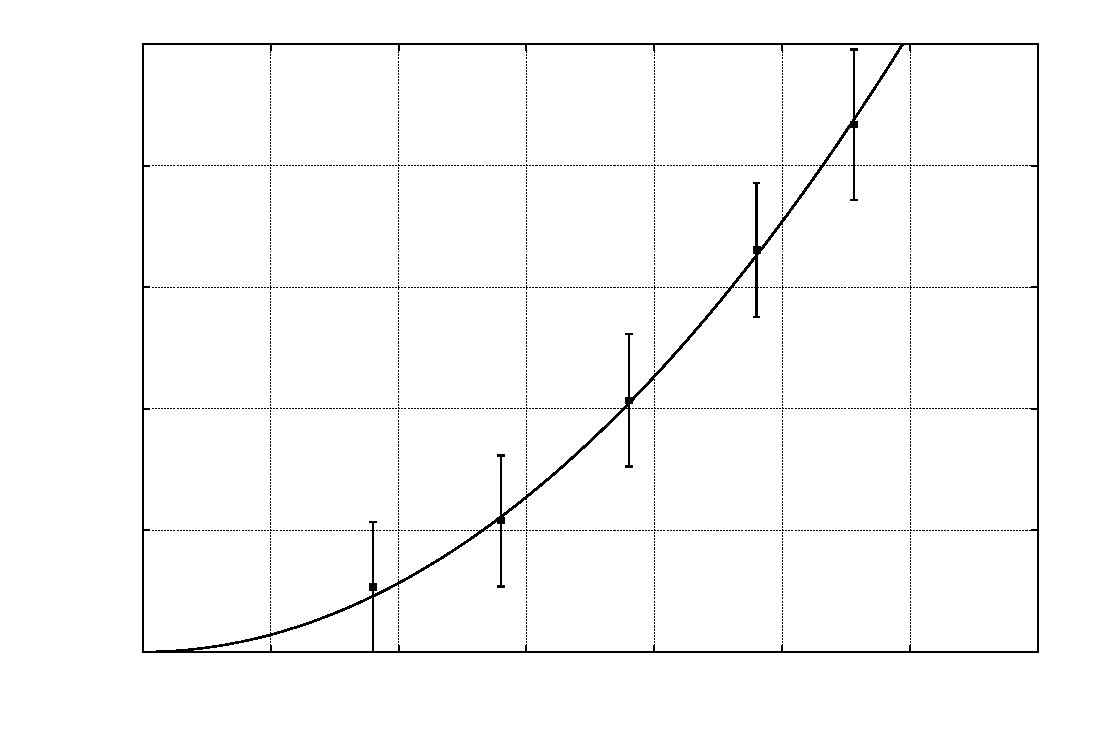
\includegraphics{graf}}%
    \gplfronttext
  \end{picture}%
\endgroup

\caption{Závislost stupně vazby $\kappa$ na vzdálenosti upevnění pružiny A od uložení závěsů kyvadel $l$}
\label{grp::kappanal}
\end{graph}



%Diskuze výsledků
\section*{Diskuze}
Teoretické hodnoty $\omega_3$ a $\omega_4$ podle vztahu \eqref{eq::omega34} jsou pro $l =$ \SI{27.8(1)}{cm}:
\begin{itemize}
\item \begin{tabbing} Pružina A: \= $\omega_3=\SI{3.52(3)}{\per\s}$	\\ \> $\omega_4=\SI{0.15(3)}{\per\s}$  \end{tabbing}
\item \begin{tabbing} Pružina B: \= $\omega_3=\SI{3.44(3)}{\per\s}$	\\ \> $\omega_4=\SI{0.08(3)}{\per\s}$  \end{tabbing}
\end{itemize}

Všechny naměřené hodnoty se velmi přesně shodují s teoretickými, až na $\omega_3$ s pružinou A (naměřeno \SI{2.96(3)}{\per\s}), která se od teoretické výrazně liší.
Vzhledem k tomu, že naměřené $\omega_4$ velmi přesně odpovídá naměřeným $\omega_1$ a $\omega_2$, je nejpravděpodobnější příčinou hrubá chyba při měření periody $T_3$ (pravděpodobně chybný odečet počtu měřených period).
Nemůžeme ale vyloučit, že se o hrubou chybu nejedná a pohyb kyvadel našemu modelu neodpovídá.
V každém případě je měření neprůkazné a mělo by se zopakovat.

Pokud upevníme pružinu s tuhostí $k$ ve vzdálenosti $l$ od upevnění kyvadla, působí při malých výchylkách (tj.~$\sin (\varphi) \approx \varphi$) na kyvadlo silou
\begin{equation}
F=-k \cdot l \cdot \varphi
\end{equation}
a působí momentem síly $M = F \cdot l$
\begin{equation}
M = -k \cdot l^2 \cdot \varphi  \,.
\end{equation}

Porovnáním s definicí direkčního momentu
\begin{equation}
M = -D \cdot \varphi
\end{equation}
snadno nahlédneme, že pro direkční moment pružiny $D^{\ast}$ platí
\begin{equation}
D^{\ast} = -k \cdot l^2 \,.
\end{equation}

Dosazením do \eqref{eq::kappadirekcni} dostáváme pro slabé vazby a krátké vzdálenosti $l$ (tj.~$D^{\ast} \ll D$)
\begin{equation}
\kappa = a \cdot l^2 \,,
\end{equation}
kde $a = D^{\ast}/D$. Proto jsme v grafu \ref{grp::kappanal} fitovali závislost funkcí $\kappa(l)=a \cdot l^2$. Všechny hodnoty leží velmi přesně na této křivce.


%Závěr
\section*{Závěr}
Změřili jsme dobu kmitu dvou nevázaných fyzických kyvadel, hodnoty jsou uvedeny v tabulce \ref{tab::nevazany}.

Dále jsme měřili periody těchto kyvadel při vazbě různými pružinami upevněnými v různých vzdálenostech od uložení závěsů a při různých počátečních podmínkách.
Naměřené doby kmitů $T_1$, $T_2$, $T_3$ a $T_S$ pro $l = \SI{27.8(1)}{\cm}$ jsou uvedeny v tabulce \ref{tab::vsechnyomegy}.
Teoretický vztah \eqref{eq::omega34} nesplňuje pouze $\omega_3$ pro pružinu A, tato hodnota je pravděpodobně zatížena hrubou chybou.

Dále jsme s pružinou A měřili závislost stupně vazby na vzdálenosti jejího upevnění od uložení závěsů kyvadel.
Naměřené hodnoty jsou uvedeny v tabulce \ref{tab::pruzinaAruznyl} a vyneseny do grafu \ref{grp::kappanal}.
Hodnoty téměř dokonale kopírují teoretickou závislost pro slabé vazby $\kappa = a \cdot l^2$.


\printbibliography[title={Seznam použité literatury}]

\end{document}